\section{Código gerado}

Criamos um back-end do compilador para a geração do código. 
A linguagem usada na criação do código intermediário é uma restrição da linguagem C que permite usar apenas os seguintes elementos:
\begin{itemize}
	\item Expressões aritméticas, lógicas, relacionais e chamadas de funções.
	\item Todos os tipos de dados da linguagem.
	\item Todas as declarações da linguagem.
	\item Apenas os seguintes comandos de C:
	\begin{itemize}
		\item Abertura e fechamento de blocos;
		\item Sequenciamento de comandos;
		\item Atribuição;
		\item Chamadas de funções/procedimentos (incluindo de entrada e saída);
		\item Rótulos (labels) e comando goto;
		\item Comandos return, break e exit;
		\item Comandos de seleção APENAS da forma:
		\begin{itemize}
			\item \begin{verbatim}
			if( condição ) goto l;
			\end{verbatim}
			\item \begin{verbatim}
		switch ( expressão ) {
		case valor : { … }
		…
		}
		\end{verbatim}
		\item Nenhum outro comando da linguagem deve ser usado, isto inclui comandos de iteração ou de
		seleção estruturados.
		\end{itemize}
	\end{itemize}
\end{itemize}

Ao compilar um arquivo $.pie$ (como descrito em \ref{ch:uso}), um código intermediário é criado na pasta $generated\_code$ com o mesmo nome do arquivo de input, porém com a extensão $.c$. Esse arquivo pode ser compilado através do compilador $gcc$, por exemplo:
\begin{verbatim}
gcc <nomedoarquivo>.c -o <nomedoexecutavel>
\end{verbatim}


\section{Gramática de atributos}
Os atributos que os símbolos podem ter são:
\begin{center}
\begin{tabular}{|c|c|}
\hline
    cs & código do programa a ser gerado\\ \hline
    st & tabela de símbolos \\ \hline
    type & tipo \\ \hline
    ids & list de ids \\ \hline
    arraybody & parte do código que fica dentro de `[' `]' quando declarando ou acessando arrays\\ \hline
    ra & struct com índices inicial e final e de um range \\ \hline
    ids\_info & informação auxiliar para os ids, dizendo de qual tipo são \\ \hline
    id\_token & o token do id, que precisa ser passado para regras onde ele fica separado \\ \hline
    afterlabel & label que vem depois de um loopblock para ser referenciadas por gotos \\ \hline
\end{tabular}
\end{center}


A Tabela \ref{atributos} mostra os atributos de cada símbolos. Os atributos sintetizados estarão em \sintetizado{azul} e os herdados em \herdado{vermelho}.

\begin{center}
\begingroup
\begin{longtable}{l|l|}
\caption{Atributos}
\label{atributos}\\
 \hline
\multicolumn{1}{|L{5cm}|}{\textbf{NÃO TERMINAIS}} & \textbf{ATRIBUTOS}                                                                      \\ \hline
\multicolumn{1}{|L{5cm}|}{PROGRAM}            & \sintetizado{cs}                                                                      \\ \hline
\multicolumn{1}{|L{5cm}|}{DECL}               & {\color[HTML]{000000} \sintetizado{cs}, \sintetizado{st}}  \\ \hline
\multicolumn{1}{|L{5cm}|}{CONSTS}             & \sintetizado{cs}, \sintetizado{st}                         \\ \hline
\multicolumn{1}{|L{5cm}|}{LISTCONST}          & \sintetizado{cs}, \sintetizado{st}                         \\ \hline
\multicolumn{1}{|L{5cm}|}{LISTCONSTPRIME}     & \sintetizado{cs}, \sintetizado{st}                         \\ \hline
\multicolumn{1}{|L{5cm}|}{CONSTDECL}          & \sintetizado{cs}, \sintetizado{st}                         \\ \hline
\multicolumn{1}{|L{5cm}|}{TYPES}              & \sintetizado{cs}, \sintetizado{st}, \herdado{st}, \sintetizado{type}, \sintetizado{arraybody} \\ \hline
\multicolumn{1}{|L{5cm}|}{TYPESPRIME}         & \sintetizado{cs}                                                                      \\ \hline
\multicolumn{1}{|L{5cm}|}{PRIMTYPES}          & \sintetizado{cs}, \sintetizado{type}, \sintetizado{st}, \sintetizado{arraybody}      \\ \hline
\multicolumn{1}{|L{5cm}|}{ARRAYTYPE}          & \sintetizado{cs}, \sintetizado{st}, \sintetizado{arraybody}             \\ \hline
\multicolumn{1}{|L{5cm}|}{SUBRANGELIST}       & \sintetizado{ra}                                                                      \\ \hline
\multicolumn{1}{|L{5cm}|}{SUBRANGEPART}       & \sintetizado{ra}                                                                      \\ \hline
\multicolumn{1}{|L{5cm}|}{SUBRANGEPARTPRIME}  & \sintetizado{ra}                                                                      \\ \hline
\multicolumn{1}{|L{5cm}|}{SUBRANGETYPE2}      & \sintetizado{ra}                                                                      \\ \hline
\multicolumn{1}{|L{5cm}|}{ENUMTYPE}           & \sintetizado{cs}                                                                      \\ \hline
\multicolumn{1}{|L{5cm}|}{RECORDTYPE}         & \sintetizado{cs}, \sintetizado{st}                         \\ \hline
\multicolumn{1}{|L{5cm}|}{USERTYPES}          & \sintetizado{cs}, \sintetizado{st}                         \\ \hline
\multicolumn{1}{|L{5cm}|}{LISTUSERTYPES}      & \sintetizado{cs}, \sintetizado{st}                         \\ \hline
\multicolumn{1}{|L{5cm}|}{LISTUSERTYPESPRIME} & \sintetizado{cs}, \sintetizado{st}                         \\ \hline
\multicolumn{1}{|L{5cm}|}{USERTYPE}           & \sintetizado{cs}, \sintetizado{st}                         \\ \hline
\multicolumn{1}{|L{5cm}|}{VARS}               & \sintetizado{cs}, \sintetizado{st}                         \\ \hline
\multicolumn{1}{|L{5cm}|}{VARLISTLIST}        & \sintetizado{cs}, \sintetizado{st}                         \\ \hline
\multicolumn{1}{|L{5cm}|}{VARLISTLISTPRIME}   & \sintetizado{cs}, \sintetizado{st}                         \\ \hline
\multicolumn{1}{|L{5cm}|}{VARLIST}            & \sintetizado{cs}, \sintetizado{st}                         \\ \hline
\multicolumn{1}{|L{5cm}|}{IDLIST}             & \sintetizado{cs}, \sintetizado{ids},  \herdado{ids\_info}            \\ \hline
\multicolumn{1}{|L{5cm}|}{IDLISTPRIME}        & \sintetizado{cs}, \sintetizado{ids},  \herdado{ids\_info}            \\ \hline
\multicolumn{1}{|L{5cm}|}{IDATTR}             & cs                                                                      \\ \hline
\multicolumn{1}{|L{5cm}|}{VARIABLE}           & \sintetizado{cs}, \herdado{st}, \sintetizado{type},  \herdado{id\_token}      \\ \hline
\multicolumn{1}{|L{5cm}|}{VARIABLEPRIME}      & \sintetizado{cs}, \herdado{st}, \sintetizado{type}, \herdado{id\_token}      \\ \hline
\multicolumn{1}{|L{5cm}|}{BLOCK}              & \sintetizado{cs}, \herdado{st}, \herdado{afterlabel}            \\ \hline
\multicolumn{1}{|L{5cm}|}{STMTS}              & \sintetizado{cs}, \herdado{st}, \herdado{afterlabel}            \\ \hline
\multicolumn{1}{|L{5cm}|}{STMTLISTPRIME}      & \sintetizado{cs}, \herdado{st}, \herdado{afterlabel}            \\ \hline
\multicolumn{1}{|L{5cm}|}{STMT}               & \sintetizado{cs}, \herdado{st}, \herdado{afterlabel}            \\ \hline
\multicolumn{1}{|L{5cm}|}{STMTPRIME}          & \sintetizado{cs}, \herdado{st}                         \\ \hline
\multicolumn{1}{|L{5cm}|}{SUBPROGCALL}        & \sintetizado{cs}                                                                      \\ \hline
\multicolumn{1}{|L{5cm}|}{EXITSTMT}           & \sintetizado{cs}, \herdado{st}, \herdado{afterlabel}            \\ \hline
\multicolumn{1}{|L{5cm}|}{RETURNSTMT}         & \sintetizado{cs}                                                                      \\ \hline
\multicolumn{1}{|L{5cm}|}{ATTRSTMT}           & \sintetizado{cs}                                                                      \\ \hline
\multicolumn{1}{|L{5cm}|}{IFBLOCK}            & \sintetizado{cs}, \herdado{st}                         \\ \hline
\multicolumn{1}{|L{5cm}|}{ELSEBLOCK}          & \sintetizado{cs}, \herdado{st}                         \\ \hline
\multicolumn{1}{|L{5cm}|}{LOOPBLOCK}          & \sintetizado{cs}, \herdado{st}                         \\ \hline
\multicolumn{1}{|L{5cm}|}{CASEBLOCK}          & \sintetizado{cs}, \herdado{st}                         \\ \hline
\multicolumn{1}{|L{5cm}|}{CASEBLOCKPRIME}     & \sintetizado{cs}, \herdado{st}                         \\ \hline
\multicolumn{1}{|L{5cm}|}{CASELIST}           & \sintetizado{cs}, \herdado{st}                         \\ \hline
\multicolumn{1}{|L{5cm}|}{LITERALLIST}        & \sintetizado{cs}, \herdado{st}                         \\ \hline
\multicolumn{1}{|L{5cm}|}{LITERALLISTPRIME}   & \sintetizado{cs}, \herdado{st}                         \\ \hline
\multicolumn{1}{|L{5cm}|}{GOTOSTMT}           & cs                                                                      \\ \hline
\multicolumn{1}{|L{5cm}|}{FORBLOCK}           & \sintetizado{cs}, \herdado{st}                         \\ \hline
\multicolumn{1}{|L{5cm}|}{FORBLOCKPRIME}      & \sintetizado{cs}, \herdado{st}, \herdado{id\_token}             \\ \hline
\multicolumn{1}{|L{5cm}|}{EXPR}               & \sintetizado{cs}, \herdado{st}, \sintetizado{type}                  \\ \hline
\multicolumn{1}{|L{5cm}|}{FINAL\_TERM}        & \sintetizado{cs}, \herdado{st}, \sintetizado{type}                  \\ \hline
\multicolumn{1}{|L{5cm}|}{FINAL\_TERMPRIME}   & \sintetizado{cs}, \herdado{st}, \sintetizado{type}, \herdado{id\_token}      \\ \hline
\multicolumn{1}{|L{5cm}|}{DISJ}               & \sintetizado{cs}, \herdado{st}, \sintetizado{type}                  \\ \hline
\multicolumn{1}{|L{5cm}|}{CONJ}               & \sintetizado{cs}, \herdado{st}, \sintetizado{type}                  \\ \hline
\multicolumn{1}{|L{5cm}|}{CONJPRIME}          & \sintetizado{cs}, \herdado{st}, \sintetizado{type}                  \\ \hline
\multicolumn{1}{|L{5cm}|}{COMP}               & \sintetizado{cs}, \herdado{st}, \sintetizado{type}                  \\ \hline
\multicolumn{1}{|L{5cm}|}{RELATIONAL}         & \sintetizado{cs}, \herdado{st}, \sintetizado{type}                  \\ \hline
\multicolumn{1}{|L{5cm}|}{RELATIONALPRIME}    & \sintetizado{cs}, \herdado{st}, \sintetizado{type}                  \\ \hline
\multicolumn{1}{|L{5cm}|}{COMPPRIME}          & \sintetizado{cs}, \herdado{st}, \sintetizado{type}                  \\ \hline
\multicolumn{1}{|L{5cm}|}{SUM}                & \sintetizado{cs}, \herdado{st}, \sintetizado{type}                  \\ \hline
\multicolumn{1}{|L{5cm}|}{SUMPRIME}           & \sintetizado{cs}, \herdado{st}, \sintetizado{type}                  \\ \hline
\multicolumn{1}{|L{5cm}|}{NEG}                & \sintetizado{cs}, \herdado{st}, \sintetizado{type}                  \\ \hline
\multicolumn{1}{|L{5cm}|}{MUL}                & \sintetizado{cs}, \herdado{st}, \sintetizado{type}                  \\ \hline
\multicolumn{1}{|L{5cm}|}{MULPRIME}           & \sintetizado{cs}, \herdado{st}, \sintetizado{type}                  \\ \hline
\multicolumn{1}{|L{5cm}|}{ADD\_OP}            & \sintetizado{cs}                                                                      \\ \hline
\multicolumn{1}{|L{5cm}|}{MUL\_OP}            & \sintetizado{cs}                                                                      \\ \hline
\multicolumn{1}{|L{5cm}|}{EQUALITY\_OP}       & \sintetizado{cs}                                                                      \\ \hline
\multicolumn{1}{|L{5cm}|}{RELATIONAL\_OP}     & \sintetizado{cs}                                                                      \\ \hline
\multicolumn{1}{|L{5cm}|}{LITERAL}            & \sintetizado{cs}, \sintetizado{type}                       \\ \hline
\multicolumn{1}{|L{5cm}|}{EXPRLIST}           & \sintetizado{cs}                                                                      \\ \hline
\multicolumn{1}{|L{5cm}|}{EXPRLISTPLUS}       & \sintetizado{cs}                                                                      \\ \hline
\multicolumn{1}{|L{5cm}|}{EXPRLISTPLUSPRIME}  & \sintetizado{cs}                                                                      \\ \hline
\multicolumn{1}{|L{5cm}|}{SUBPROGRAMS}        & \sintetizado{cs}, \herdado{st}                         \\ \hline
\multicolumn{1}{|L{5cm}|}{SUBPROGRAMSPRIME}   & \sintetizado{cs}, \herdado{st}                         \\ \hline
\multicolumn{1}{|L{5cm}|}{PROCEDURE}          & \sintetizado{cs}, \herdado{st}                         \\ \hline
\multicolumn{1}{|L{5cm}|}{FUNCTION}           & \sintetizado{cs}, \herdado{st}                         \\ \hline
\multicolumn{1}{|L{5cm}|}{PARAM}              & \sintetizado{cs}, \sintetizado{st}                         \\ \hline
\multicolumn{1}{|L{5cm}|}{PARAMLISTLIST}      & \sintetizado{cs}, \sintetizado{st}                         \\ \hline
\multicolumn{1}{|L{5cm}|}{PARAMLISTLISTPRIME} & \sintetizado{cs}, \sintetizado{st}                         \\ \hline
\multicolumn{1}{|L{5cm}|}{PARAMLIST}          & \sintetizado{cs}, \sintetizado{st}                         \\ \hline
\multicolumn{1}{|L{5cm}|}{WRITESTMT}          & \sintetizado{cs}, \herdado{st}                         \\ \hline
\multicolumn{1}{|L{5cm}|}{WRITELNSTMT}        & \sintetizado{cs}, \herdado{st}                         \\ \hline
\multicolumn{1}{|L{5cm}|}{READSTMT}           & \sintetizado{cs}, \herdado{st}                         \\ \hline
\multicolumn{1}{|L{5cm}|}{READLNSTMT}         & \sintetizado{cs}, \herdado{st}                         \\ \hline
\end{longtable}
\endgroup
\end{center}


\newpage
\subsection{Grafo de Dependência}

A imagem a seguir apresenta o grafo de dependência para a regra do procedimento.

\begin{lstlisting}%[\scriptsize, frame=single, language=pie]
<procedure> ::= proc id '(' <param> ')' ';' <decl> <block>
\end{lstlisting}

\begin{figure}[H]
  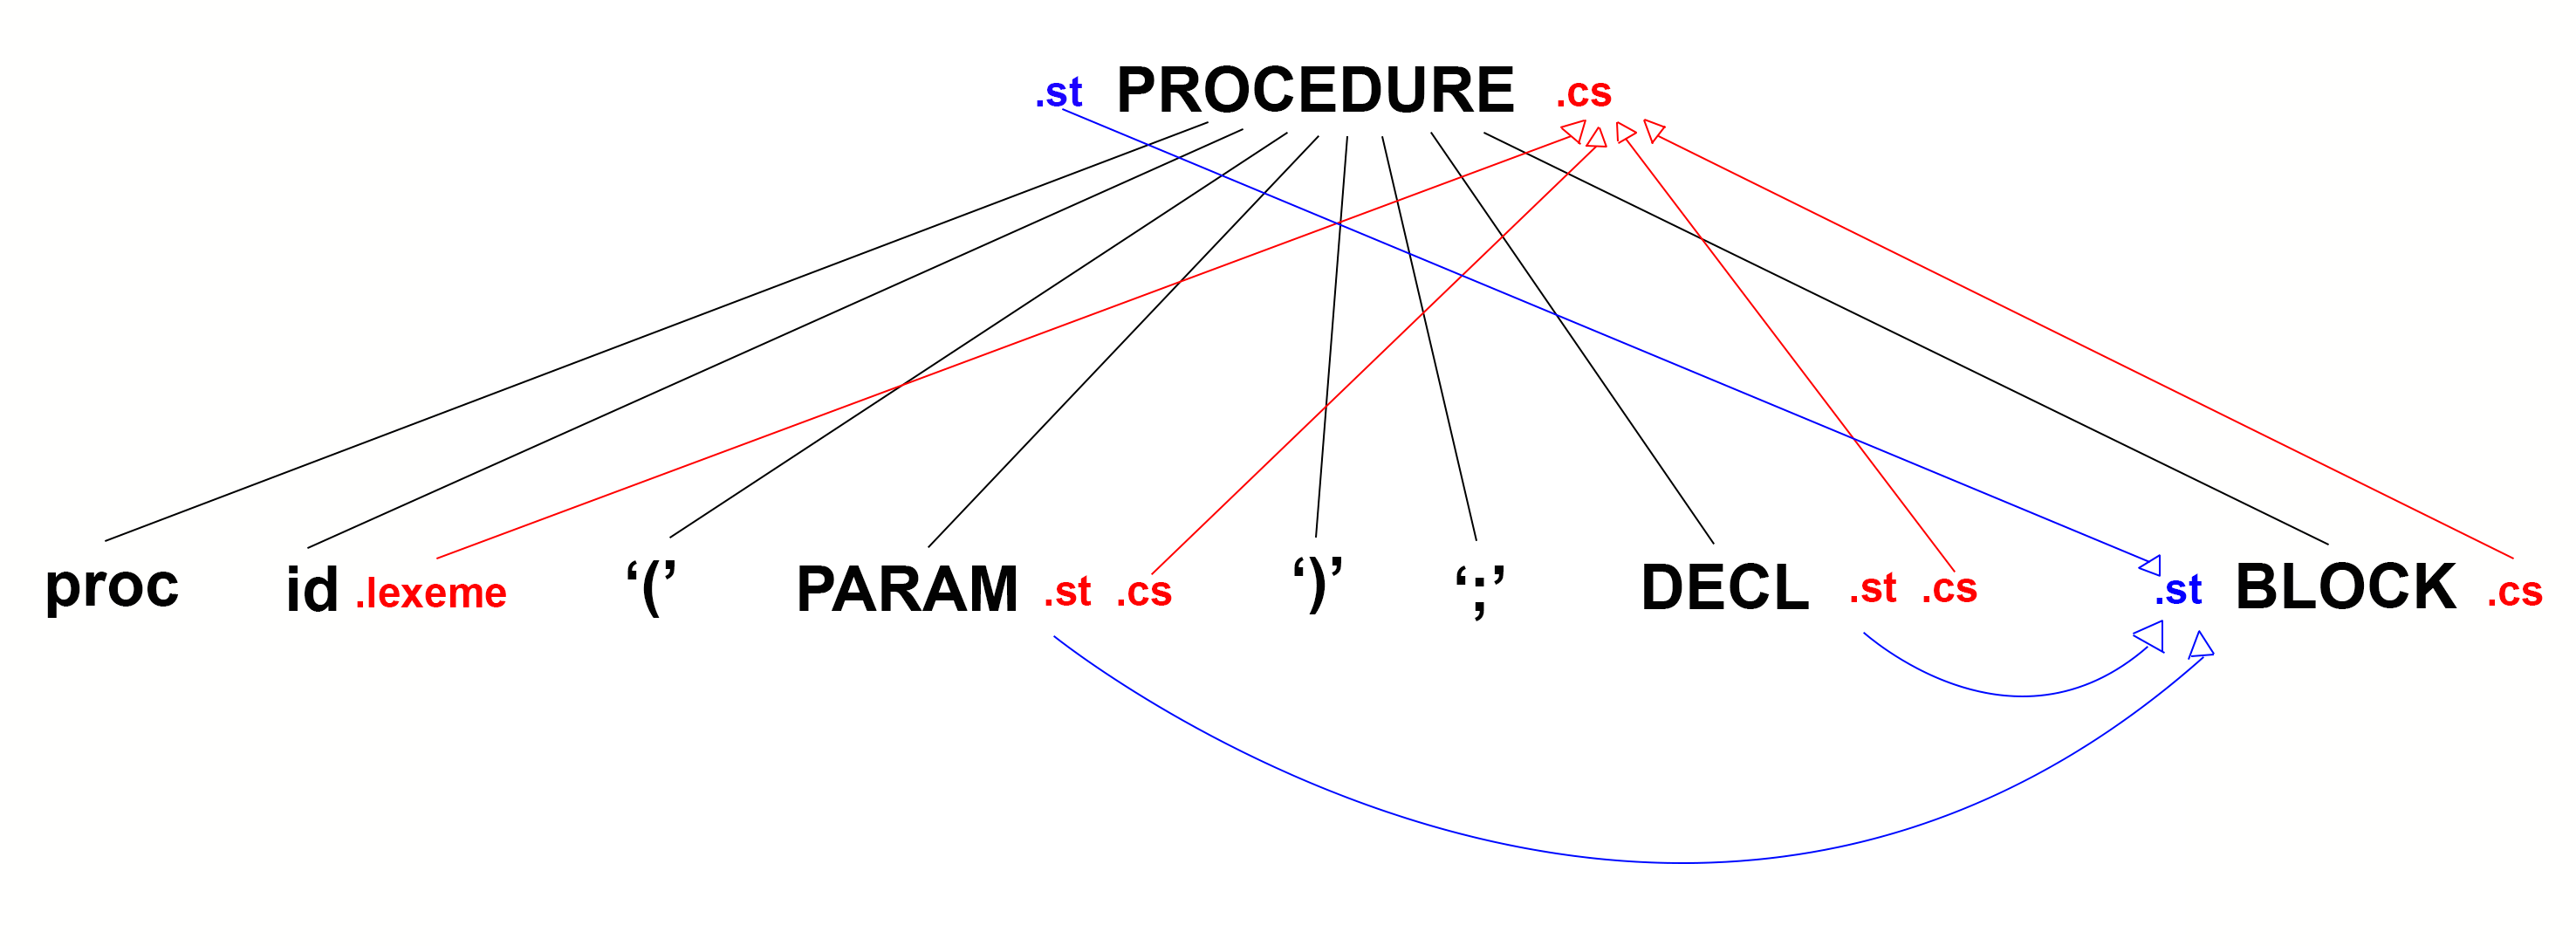
\includegraphics[width=\textwidth]{img/dependency_graph.png}
  \caption{Grafo de dependência para a regra de produção de PROCEDURE}
  \label{fig:dependencegraph}
\end{figure}

O código a seguir é a implementação da regra do procedimento baseada na gramática de atributos.

\begin{verbbox}[\scriptsize]
    {BLOCK.st =st_union(PARAM.st,st_union(DECL.st,PROCEDURE.st));
    PROCEDURE.cs = "void " + id.lexeme + "(" + PARAM.cs + ") {\n" + DECL.cs + BLOCK.cs + "\n}\n"; }
\end{verbbox}
\theverbbox


\subsubsection{Gramática de Atributos}
Operações usadas:

%\lstset{language=C,
                %keywordstyle=\color{blue},
                %stringstyle=\color{red},
                %commentstyle=\color{green} morecomment=[l][\color{magenta}]{\#}
%}
%\begin{footnotesize}
%\lstinputlisting[language=C]{backend/funcoes.c}
%\end{footnotesize}
%\lstset{language=pie}
{\scriptsize\verbatiminput{backend/funcoes.c}}

Gramática de atributos:\\

\begin{verbbox}[\scriptsize]
PROGRAM -> 'program' 'id' ';' DECL BLOCK '.'
{
BLOCK.st = DECL.st; PROGRAM.cs = includes() +
"typedef int bool;\n#define true 1\n#define false 0\n\n" +
DECL.cs + "int main() {\n" + BLOCK.cs + "\nreturn 0;\n}\n";
}
\end{verbbox}
\theverbbox\\

\begin{verbbox}[\scriptsize]
DECL -> CONSTS USERTYPES VARS SUBPROGRAMS
{
SUBPROGRAMS.st = union(CONSTS.st, union(USERTYPES.st, VARS.st));
DECL.st = union(CONSTS.st, union(USERTYPES.st, VARS.st));
DECL.cs = CONSTS.cs + USERTYPES.cs + VARS.cs + SUBPROGRAMS.cs;
}
\end{verbbox} 
\theverbbox\\

\begin{verbbox}[\scriptsize]
CONSTS -> '' {}
CONSTS -> 'const' LISTCONST
{
CONST.st = LISTCONST.st;
CONST.cs = LISTCONST.cs;
}
\end{verbbox} 
\theverbbox\\

\begin{verbbox}[\scriptsize]
LISTCONST -> CONSTDECL LISTCONSTPRIME
{
LISTCONST.st = union(CONSTDECL.st, LISTCONSTPRIME.st);
LISTCONST.cs = CONSTDECL.cs + LISTCONSTPRIME.cs;
}
\end{verbbox} 
\theverbbox\\

\begin{verbbox}[\scriptsize]
LISTCONSTPRIME -> '' {}
LISTCONSTPRIME -> LISTCONST
{
LISTCONSTPRIME.st = LISTCONST.st;
LISTCONSTPRIME.cs = LISTCONST.cs;
}
\end{verbbox} 
\theverbbox\\

\begin{verbbox}[\scriptsize]
CONSTDECL -> 'id' '=' EXPR ';'
{
CONSTDECL.st.st[id.lexeme] = EXPR.type;
CONSTDECL.cs  = "const " + EXPR.type + " " + id.lexeme + “ = ” +  EXPR.cs + “;\n”;
}
\end{verbbox} 
\theverbbox\\

\begin{verbbox}[\scriptsize]
TYPES -> 'id' TYPESPRIME
{
TYPES.type = TYPESPRIME.type;
TYPES.cs = id + “ “ + TYPESPRIME.cs;
}
TYPES -> PRIMTYPES
{
TYPES.type = PRIMTYPES.type;
TYPES.st = PRIMTYPES.st;
TYPES.arraybody = PRIMTYPES.arraybody;
TYPES.cs = PRIMTYPES.cs;
}
\end{verbbox} 
\theverbbox\\

\begin{verbbox}[\scriptsize]
TYPESPRIME -> '' {}
TYPESPRIME -> SUBRANGEPART
{
TYPESPRIME.cs = SUBRANGEPART.cs;
}
TYPESPRIME -> VARIABLE SUBRANGEPART
{
TYPESPRIME.cs = VARIABLE.cs + SUBRANGEPART.cs;
}
\end{verbbox} 
\theverbbox\\

\begin{verbbox}[\scriptsize]
PRIMTYPES -> 'int'
{
PRIMTYPES.type = "int";
PRIMTYPES.cs = "int";
}
PRIMTYPES -> 'real'
{
PRIMTYPES.type = "float";
PRIMTYPES.cs = "float";
}
PRIMTYPES -> 'bool'
{
PRIMTYPES.type = "bool";
PRIMTYPES.cs = "bool";
}
PRIMTYPES -> 'char'
{
PRIMTYPES.type = "char";
PRIMTYPES.cs = "char";
}
PRIMTYPES -> 'string'
{
PRIMTYPES.type = "char*";
PRIMTYPES.cs = "char*";
}
PRIMTYPES -> ARRAYTYPE
{
PRIMTYPES.type = "array";
PRIMTYPES.st = ARRAYTYPE.st;
PRIMTYPES.arraybody = ARRAYTYPE.arraybody;
PRIMTYPES.cs = ARRAYTYPE.cs;
}
PRIMTYPES -> SETTYPE
{
PRIMTYPES.type = "set";
PRIMTYPES.cs = SETTYPE.cs;
}
PRIMTYPES -> ENUMTYPE
{PRIMTYPES.type = "enum";
PRIMTYPES.cs = ENUMTYPE.cs;
}
PRIMTYPES -> RECORDTYPE
{
PRIMTYPES.type = "struct";
PRIMTYPES.st = RECORDTYPE.st;
PRIMTYPES.cs = RECORDTYPE.cs;
}
PRIMTYPES -> SUBRANGETYPE2 SUBRANGEPART
{
PRIMTYPES.type = "subrange";
PRIMTYPES.cs = SUBRANGETYPE2.cs + SUBRANGEPART.cs;
}
\end{verbbox} 
\theverbbox\\

\begin{verbbox}[\scriptsize]
ARRAYTYPE -> 'array' '[' SUBRANGELIST ']' 'of' TYPES
{
ArrayAttrs aa; aa.type = TYPES.type; aa.init_idx = SUBRANGELIST.ra.init_idx; 
ARRAYTYPE.st.array_STs.push_back(aa); 
ARRAYTYPE.arraybody = "[" + std::to_string(SUBRANGELIST.ra.end_idx - SUBRANGELIST.ra.init_idx + 1) + "]"; 
ARRAYTYPE.cs = TYPES.type;
}
\end{verbbox} 
\theverbbox\\

\begin{verbbox}[\scriptsize]
SUBRANGELIST -> SUBRANGETYPE2 SUBRANGEPART SUBRANGELISTPRIME
{
SUBRANGELIST.ra.init_idx = SUBRANGETYPE2.ra.init_idx; 
SUBRANGELIST.ra.end_idx = SUBRANGEPART.ra.end_idx;
}
SUBRANGELIST -> SUBRANGETYPE1 SUBRANGELISTTYPE1
\end{verbbox} 
\theverbbox\\

\begin{verbbox}[\scriptsize]
SUBRANGELISTTYPE1 -> SUBRANGEPART SUBRANGELISTPRIME
SUBRANGELISTTYPE1 -> SUBRANGELISTPRIME
\end{verbbox} 
\theverbbox\\

\begin{verbbox}[\scriptsize]
SUBRANGEPART -> '..' SUBRANGEPARTPRIME
{
SUBRANGEPART.ra.init_idx = SUBRANGEPARTPRIME.ra.init_idx; 
SUBRANGEPART.ra.end_idx = SUBRANGEPARTPRIME.ra.end_idx;
}
\end{verbbox} 
\theverbbox\\

\begin{verbbox}[\scriptsize]
SUBRANGEPARTPRIME -> SUBRANGETYPE1
SUBRANGEPARTPRIME -> SUBRANGETYPE2
{
SUBRANGEPARTPRIME.ra.init_idx = SUBRANGETYPE2.ra.init_idx; 
SUBRANGEPARTPRIME.ra.end_idx = SUBRANGETYPE2.ra.end_idx;
}
\end{verbbox} 
\theverbbox\\

\begin{verbbox}[\scriptsize]
SUBRANGELISTPRIME -> '' {}
SUBRANGELISTPRIME -> ',' SUBRANGELIST
\end{verbbox} 
\theverbbox\\

\begin{verbbox}[\scriptsize]
SUBRANGETYPE1 -> 'id' SUBRANGETVARPART
\end{verbbox}
\theverbbox\\

\begin{verbbox}[\scriptsize]
SUBRANGETYPE2 -> 'intliteral'
{
SUBRANGETYPE2.ra.init_idx = std::stoi(intliteral.val);
SUBRANGETYPE2.ra.end_idx = std::stoi(intliteral.val);
}
SUBRANGETYPE2 -> 'charliteral'
\end{verbbox}
\theverbbox\\

\begin{verbbox}[\scriptsize]
SUBRANGETVARPART -> '' {}
SUBRANGETVARPART -> VARIABLE
\end{verbbox}
\theverbbox\\

\begin{verbbox}[\scriptsize]
SETTYPE -> 'set' 'of' TYPES
\end{verbbox}
\theverbbox\\

\begin{verbbox}[\scriptsize]
ENUMTYPE -> '(' IDLIST ')'
{
ENUMTYPE.cs = "enum {" + IDLIST.cs + "}";
}
\end{verbbox}
\theverbbox\\

\begin{verbbox}[\scriptsize]
RECORDTYPE -> 'record' VARLISTLIST 'end'
{
RECORDTYPE.st = VARLISTLIST.st;
RECORDTYPE.st.struct_STs.push_back(RECORDTYPE.st.st);
RECORDTYPE.st.st.clear();
RECORDTYPE.cs = "struct {\n" + VARLISTLIST.cs + "\n}";
}
\end{verbbox}
\theverbbox\\

\begin{verbbox}[\scriptsize]
USERTYPES -> '' {}
USERTYPES -> 'type' LISTUSERTYPES
{
USERTYPES.st = LISTUSERTYPES.st;
USERTYPES.cs  = LISTUSERTYPES.cs;
}
\end{verbbox}
\theverbbox\\

\begin{verbbox}[\scriptsize]
LISTUSERTYPES -> USERTYPE LISTUSERTYPESPRIME
{
LISTEUSERTYPES.st = union(USERTYPE.st, LISTUSERTYPESPRIME.st);
LISTUSERTYPES.cs = USERTYPE.cs + LISTUSERTYPESPRIME.cs;
}
\end{verbbox}
\theverbbox\\

\begin{verbbox}[\scriptsize]
LISTUSERTYPESPRIME -> '' {}
LISTUSERTYPESPRIME -> LISTUSERTYPES
{
LISTUSERTYPESPRIME.st = LISTUSERTYPES.st;
LISTUSERTYPESPRIME.cs = LISTUSERTYPES.cs
}
\end{verbbox}
\theverbbox\\

\begin{verbbox}[\scriptsize]
USERTYPE -> 'id' '=' TYPES ';'
{
USERTYPE.st.st[id.lexeme] = TYPES.type; 
if(TYPES.type == "struct") {
    USERTYPE.st.struct_STs = TYPES.st.struct_STs;
    USERTYPE.st.struct_ST_idx[id.lexeme] = USERTYPE.st.struct_STs.size() - 1;
} else if(TYPES.type == "array") {
    USERTYPE.st.array_STs = TYPES.st.array_STs;
    USERTYPE.st.array_ST_idx[id.lexeme] = USERTYPE.st.array_STs.size() - 1;
}
if (TYPES.type == "array") {
    USERTYPE.cs = "typedef " + TYPES.cs + " " + id.lexeme + TYPES.arraybody + ";\n";
} else {
    USERTYPE.cs = "typedef " + TYPES.cs + " " + id.lexeme + ";\n";
}
}
\end{verbbox}
\theverbbox\\

\begin{verbbox}[\scriptsize]
VARS -> '' {}
VARS -> 'var' VARLISTLIST
{
VARS.st = VARLISTLIST.st;
VARS.cs = VARLISTLIST.cs;
}
\end{verbbox}
\theverbbox\\

\begin{verbbox}[\scriptsize]
VARLISTLIST -> VARLIST VARLISTLISTPRIME
{
VARLISTLIST.st = union(VARLIST.st, VARLISTLISTPRIME.st);
VARLISTLIST.cs = VARLIST.cs + VARLISTLISTPRIME.cs;
}
\end{verbbox}
\theverbbox\\

\begin{verbbox}[\scriptsize]
VARLISTLISTPRIME -> '' {}
VARLISTLISTPRIME -> VARLISTLIST
{
VARLISTLISTPRIME.st = VARLISTLIST.st;
VARLISTLISTPRIME.cs = VARLISTLIST.cs;
}
\end{verbbox}
\theverbbox\\

\begin{verbbox}[\scriptsize]
VARLIST -> TYPES IDLIST ';'
{
IDLIST.ids_info.type = "var";
VARLIST.st.st = addIds(TYPES.type, IDLIST.ids);
if(TYPES.type == "struct") {
    VARLIST.st.struct_STs = TYPES.st.struct_STs;
    for(int i = 0; i < IDLIST.ids.size(); i++) {
        VARLIST.st.struct_ST_idx[IDLIST.ids[i]] = VARLIST.st.struct_STs.size() - 1;
    }
} else if(TYPES.type == "array") {
    VARLIST.st.array_STs = TYPES.st.array_STs;
    for(int i = 0; i < IDLIST.ids.size(); i++) {
        VARLIST.st.array_ST_idx[IDLIST.ids[i]] = VARLIST.st.array_STs.size() - 1;
    }
}
if (TYPES.type == "array") {
    VARLIST.cs = TYPES.cs + " ";
    for(int i = 0; i < IDLIST.ids.size(); ) {
        VARLIST.cs += IDLIST.ids[i] + TYPES.arraybody;
        i++;
        if (i == IDLIST.ids.size()) {
            VARLIST.cs += ";\n";
        } else {
            VARLIST.cs += ", ";
        }
    }
} else {
    VARLIST.cs = TYPES.cs + " " + IDLIST.cs + ";\n";
}
}
\end{verbbox}
\theverbbox\\

\begin{verbbox}[\scriptsize]
IDLIST -> 'id' IDATTR IDLISTPRIME
{
IDLISTPRIME.ids_info = IDLIST.ids_info;
IDLIST.ids = IDLISTPRIME.ids; 
IDLIST.ids.push_back(id.lexeme);
if(IDLIST.ids_info.type == "var") {
    IDLIST.cs = id.lexeme + IDATTR.cs + IDLISTPRIME.cs;
} else {
    IDLIST.cs = IDLIST.ids_info.type + " " + id.lexeme + IDATTR.cs + IDLISTPRIME.cs;
}
}
\end{verbbox}
\theverbbox\\

\begin{verbbox}[\scriptsize]
IDLISTPRIME -> '' {}
IDLISTPRIME -> ',' IDLIST
{
IDLIST.ids_info =  IDLISTPRIME.ids_info;
IDLISTPRIME.st = IDLIST.st;
IDLISTPRIME.ids = IDLIST.ids;
IDLISTPRIME.cs = ", " + IDLIST.cs;
}
\end{verbbox}
\theverbbox\\

\begin{verbbox}[\scriptsize]
IDATTR -> '' {}
IDATTR -> '=' EXPR
{
IDATTR.cs = " = " + EXPR.cs;
}
\end{verbbox}
\theverbbox\\

\begin{verbbox}[\scriptsize]
VARIABLE -> '->' 'id' VARIABLEPRIME
{
VARIABLEPRIME.st = VARIABLE.st;
VARIABLEPRIME.id_token = VARIABLE.id_token;
VARIABLE.type = VARIABLE.st.struct_STs[VARIABLE.st.struct_ST_idx[VARIABLE.id_token]][id.lexeme]; 
VARIABLE.cs = "." + id.lexeme + VARIABLEPRIME.cs;
}
VARIABLE -> '[' EXPRLISTPLUS ']' VARIABLEPRIME
{
VARIABLEPRIME.st = VARIABLE.st;
VARIABLEPRIME.id_token = VARIABLE.id_token;
VARIABLE.type = "";
VARIABLE.cs = "[" + EXPRLISTPLUS.cs + " - " + std::to_string(VARIABLE.st.
    array_STs[VARIABLE.st.array_ST_idx[VARIABLE.id_token]].init_idx) + "]" + VARIABLEPRIME.cs;
}
\end{verbbox}
\theverbbox\\

\begin{verbbox}[\scriptsize]
VARIABLEPRIME -> '' {}
VARIABLEPRIME -> VARIABLE
{
VARIABLE.id_token = VARIABLEPRIME.id_token;
VARIABLE.st = VARIABLEPRIME.st;
VARIABLEPRIME.type = VARIABLE.type;
VARIABLEPRIME.cs = VARIABLE.cs;
}
\end{verbbox}
\theverbbox\\

\begin{verbbox}[\scriptsize]
BLOCK -> 'begin' STMTS 'end'
{
STMTS.st = BLOCK.st;
BLOCK.cs = STMTS.cs;
}
\end{verbbox}
\theverbbox\\

\begin{verbbox}[\scriptsize]
STMTS -> STMT STMTLISTPRIME
{
STMT.st = STMTS.st;
STMTLISTPRIME.st = STMTS.st;
STMTS.cs = STMT.cs + ";\n" + STMTLISTPRIME.cs;
}
\end{verbbox}
\theverbbox\\

\begin{verbbox}[\scriptsize]
STMTLISTPRIME -> '' {}
STMTLISTPRIME -> ';' STMTS
{
STMTS.st = STMTLISTPRIME.st;
STMTLISTPRIME.cs = STMTS.cs;
}
\end{verbbox}
\theverbbox\\

\begin{verbbox}[\scriptsize]
STMT -> '' {}
STMT -> 'label' STMT
{
STMT_1.st = STMT_0.st;
std::string label = label.lexeme; 
label[0] = '_'; 
STMT_0.cs = label + ":\n" + STMT_1.cs;
}
STMT -> BLOCK
{
BLOCK.st = STMT.st
BLOCK.afterlabel = STMT.afterlabel;
STMT.cs = BLOCK.cs;
}
STMT -> WRITESTMT
{
WRITESTMT.st = STMT.st;
STMT.cs  = WRITESTMT.cs;
}
STMT -> WRITELNSTMT
{
WRITELNSTMT.st = STMT.st;
STMT.cs = WRITELNSTMT.cs;
}
STMT -> READSTMT
{
READSTMT.st = STMT.st;
STMT.cs = READSTMT.cs;
}
STMT -> READLNSTMT
{
READLNSTMT.st = STMT.st;
STMT.cs = READLNSTMT.cs;
}
STMT -> LOOPBLOCK
{
LOOPBLOCK.st = STMT.st;
STMT.cs = LOOPBLOCK.cs;
}
STMT -> IFBLOCK
{
IFBLOCK.st = STMT.st;
STMT.cs = IFBLOCK.cs;
}
STMT -> FORBLOCK
{
FORBLOCK.st = STMT.st;
STMT.cs = FORBLOCK.cs;
}
STMT -> CASEBLOCK
{
CASEBLOCK.st = STMT.st;
STMT.cs = CASEBLOCK.cs;
}
STMT -> GOTOSTMT
{
STMT.cs = GOTOSTMT.cs;
}
STMT -> 'id' STMTPRIME
{
STMTPRIME.st = STMT.st;
STMT.cs = id.lexeme + STMTPRIME.cs;
}
STMT -> EXITSTMT
{
EXITSTMT.st = STMT.st;
EXITSTMT.afterlabel = STMT.afterlabel;
STMT.cs = EXITSTMT.cs;
}
STMT -> RETURNSTMT
{
STMT.cs = RETURNSTMT.cs;
}
\end{verbbox}
\theverbbox\\

\begin{verbbox}[\scriptsize]
STMTPRIME -> ATTRSTMT
{
STMTPRIME.cs = ATTRSTMT.cs;
}
STMTPRIME -> SUBPROGCALL
{
STMTPRIME.cs = SUBPROGCALL.cs;
}
\end{verbbox} 
\theverbbox\\

\begin{verbbox}[\scriptsize]
SUBPROGCALL -> '(' EXPRLIST ')'
{
SUBPROGCALL.cs = “(” + EXPRLIST.cs + “);\n”;
}
\end{verbbox} 
\theverbbox\\

\begin{verbbox}[\scriptsize]
EXITSTMT -> 'exitwhen' EXPR
{
EXITSTMT.cs = "if (" + EXPR.cs + ") goto " + EXITSTMT.afterlabel + ";\n";
}
\end{verbbox} 
\theverbbox\\

\begin{verbbox}[\scriptsize]
RETURNSTMT -> 'return' EXPR
{
RETURNSTMT.cs = "return " + EXPR.cs + ";\n";
}
\end{verbbox} 
\theverbbox\\

\begin{verbbox}[\scriptsize]
ATTRSTMT -> VARIABLE ':=' EXPR
{
ATTRSTMT.cs = VARIABLE.cs + “ = ” + EXPR.cs + ";\n";
}
ATTRSTMT -> ':=' EXPR
{
ATTRSTMT.cs = “ = ” + EXPR.cs + ";\n";
}
\end{verbbox} 
\theverbbox\\

\begin{verbbox}[\scriptsize]
IFBLOCK -> 'if' EXPR STMT ELSEBLOCK
{
STMT.st = IFBLOCK.st;
ELSEBLOCK.st = IFBLOCK.st;
std::string label1 = generateNewLabel(), label2 = generateNewLabel();
IFBLOCK.cs = "if (!(" + EXPR.cs + ")) goto " + label1 + ";\n" + 
    STMT.cs + "goto " + label2 + ";\n" + label1 + ":\n" + ELSEBLOCK.cs + label2 + ":;\n";
}
\end{verbbox} 
\theverbbox\\

\begin{verbbox}[\scriptsize]
ELSEBLOCK -> '' {}
ELSEBLOCK -> 'else' STMT
{
STMT.st = ELSEBLOCK.st;
ELSEBLOCK.cs = STMT.cs;
}
\end{verbbox} 
\theverbbox\\

\begin{verbbox}[\scriptsize]
LOOPBLOCK -> 'loop' STMT
{
STMT.st = LOOPBLOCK.st;
std::string label1 = generateNewLabel(), label2 = generateNewLabel();
STMT.afterlabel = label2;
LOOPBLOCK.cs = label1 + ":\n" + STMT.cs + "\ngoto " + label1 + ";\n" + label2 + ":;\n";
}
\end{verbbox} 
\theverbbox\\

\begin{verbbox}[\scriptsize]
CASEBLOCK -> 'case' EXPR 'of' CASELIST CASEBLOCKPRIME
{
EXPR.st = CASEBLOCK.st;
CASELIST.st = CASEBLOCK.st;
CASEBLOCKPRIME.st = CASEBLOCK.st;
CASEBLOCK.cs = “switch (” + EXPR.cs + “){\n” + CASELIST.cs + CASEBLOCKPRIME.cs
}
\end{verbbox} 
\theverbbox\\

\begin{verbbox}[\scriptsize]
CASEBLOCKPRIME -> 'end'
{
CASEBLOCKPRIME.cs = “}\n”
}
CASEBLOCKPRIME -> 'else' STMT 'end'
{
STMT.st = CASEBLOCKPRIME.st;
CASEBLOCKPRIME.cs = “default: ” + STMT.cs + “;\n}\n”
}
\end{verbbox} 
\theverbbox\\

\begin{verbbox}[\scriptsize]
CASELIST -> LITERALLIST ':' STMT ';'
{
LITERALLIST.st = CASELIST.st;
STMT.st = CASELIST.st;
CASELIST.cs = LITERALLIST.cs  + “: ” + STMT.cs + “;break;\n”
}
\end{verbbox} 
\theverbbox\\

\begin{verbbox}[\scriptsize]
LITERALLIST -> LITERAL LITERALLISTPRIME
{
LITERAL.st = LITERALLIST.st;
LITERALLISTPRIME.st = LITERALLIST.st;
LITERALLIST.cs = LITERAL.cs + LITERALLISTPRIME.cs;
}
\end{verbbox} 
\theverbbox\\

\begin{verbbox}[\scriptsize]
LITERALLISTPRIME -> '' {}
LITERALLISTPRIME -> ',' LITERALLIST
{
LITERALLIST.st = LITERALLISTPRIME.st;
LITERALLLISTPRIME.cs = “,” + LITERALLIST.cs
}
\end{verbbox} 
\theverbbox\\

\begin{verbbox}[\scriptsize]
GOTOSTMT -> 'goto' 'label'
{ 
std::string label1 =  label.lexeme;
label1[0] = "_";
GOTOSTMT.cs = "goto " + label1;
}
\end{verbbox} 
\theverbbox\\

\begin{verbbox}[\scriptsize]
FORBLOCK -> 'for' 'id' FORBLOCKPRIME
{
FORBLOCKPRIME.st = FORBLOCK.st;
FORBLOCKPRIME.id_token = id.lexeme;
FORBLOCK.cs = FORBLOCKPRIMEcs;
}
\end{verbbox} 
\theverbbox\\

\begin{verbbox}[\scriptsize]
FORBLOCKPRIME -> VARIABLE ':=' EXPR\_0 'to' EXPR\_1 'step' EXPR\_2 'do' STMT
{
FORBLOCKPRIME.cs = forOutput(FORBLOCKPRIME.id_token + VARIABLE.cs, EXPR_0.cs, EXPR_1.cs,
    std::stoi(removeSpace(EXPR_2.cs)), STMT.cs);
}
FORBLOCKPRIME -> ':=' EXPR 'to' EXPR 'step' EXPR 'do' STMT
{
FORBLOCKPRIME.cs = forOutput(FORBLOCKPRIME.id_token, EXPR_0.cs, EXPR_1.cs,
    std::stoi(removeSpace(EXPR_2.cs)), STMT.cs);
}
\end{verbbox} 
\theverbbox\\

\begin{verbbox}[\scriptsize]
EXPR -> CONJ DISJ
{
CONJ.st = EXPR.st;
DISJ.st = EXPR.st;
if (DISJ.type == “nobool”) {
    EXPR.type = CONJ.type;
} else {
	EXPR.type = DISJ.type;
}
EXPR.cs = CONJ.cs + DISJ.cs
}
\end{verbbox} 
\theverbbox\\

\begin{verbbox}[\scriptsize]
FINAL_TERM -> 'id' FINAL_TERMPRIME
{
FINAL_TERMPRIME.st = FINAL_TERM.st;
FINAL_TERMPRIME.id_token = id.lexeme;
std::string type = getType(FINAL_TERM.st, id.lexeme);
if(type == "int" || type == "float" || type == "char" ||     type == "bool" || type == "char*") {
    FINAL_TERM.type = type;
} else if(type == "struct") {
    if(FINAL_TERMPRIME.type == "subprogcall") {
        FINAL_TERM.type = type;
    } else {
        FINAL_TERM.type = FINAL_TERMPRIME.type;
    }
} else if(type == "array") {
    if(FINAL_TERMPRIME.type == "subprogcall") {
        FINAL_TERM.type = type;
    } else {
        FINAL_TERM.type = getArrayType(FINAL_TERM.st, FINAL_TERM.st.array_ST_idx[id.lexeme]);
    }
}
FINAL_TERM.cs = id.lexeme + FINAL_TERMPRIME.cs;
}
FINAL_TERM -> LITERAL
{
FINAL_TERM.type = LITERAL.type;
FINAL_TERM.cs = LITERAL.cs;
}
FINAL_TERM -> '(' EXPR ')'
{
EXPR.st = FINAL_TERM.st;
FINAL_TERM.type = EXPR.type;
FINAL_TERM.cs = "(" + EXPR.cs + ")";
}
\end{verbbox} 
\theverbbox\\

\begin{verbbox}[\scriptsize]
FINAL_TERMPRIME -> VARIABLE
{
VARIABLE.st = FINAL_TERMPRIME.st;
VARIABLE.id_token = FINAL_TERMPRIME.id_token;
FINAL_TERMPRIME.type = VARIABLE.type;
FINAL_TERMPRIME.cs = VARIABLE.cs
}
FINAL_TERMPRIME -> ''
{}
FINAL_TERMPRIME -> SUBPROGCALL
{
FINAL_TERMPRIME.type = "subprogcall";
FINAL_TERMPRIME.cs = SUBPROGCALL.cs
}
\end{verbbox} 
\theverbbox\\

\begin{verbbox}[\scriptsize]
DISJ -> ''
{
DISJ.type = “nobool”;
}
DISJ -> '||' CONJ
{
CONJ.st = DISJ.st;
DISJ.type = “bool”;
DISJ.cs = “ || ” + CONJ.cs
}
\end{verbbox} 
\theverbbox\\

\begin{verbbox}[\scriptsize]
CONJ -> COMP CONJPRIME
{
COMP.st = CONJ.st;
CONJPRIME.st = CONJ.st;
if (CONJPRIME.type.compare(“nobool”)) {
    CONJ.type = COMP.type;
} else {
    CONJ.type = CONJPRIME.type;
}
CONJ.cs = COMP.cs + CONJPRIME.cs
}
\end{verbbox} 
\theverbbox\\

\begin{verbbox}[\scriptsize]
CONJPRIME -> ''
{
CONJPRIME.type = “nobool”;
}
CONJPRIME -> '&&' COMP
{
COMP.st = CONJPRIME.st;
CONJPRIME.type = “bool”;
CONJPRIME.cs = “ && ” + COMP.cs
}
\end{verbbox} 
\theverbbox\\

\begin{verbbox}[\scriptsize]
COMP -> RELATIONAL COMPPRIME
{
RELATIONAL.st = COMP.st;
COMPPRIME.st = COMP.st;
if (COMPPRIME.type == “nobool”) {
    COMP.type = RELATIONAL.type;
} else {
    COMP.type = COMPPRIME.type;
}
COMP.cs = RELATIONAL.cs + COMPPRIME.cs
}
\end{verbbox} 
\theverbbox\\

\begin{verbbox}[\scriptsize]
RELATIONAL -> SUM RELATIONALPRIME
{
SUM.st = RELATIONAL.st;
RELATIONALPRIME.st = RELATIONAL.st;
if (RELATIONALPRIME.type == “nobool”) {
    RELATIONAL.type = SUM.type;
} else {
    RELATIONAL.type = RELATIONALPRIME.type;
}
RELATIONAL.cs = SUM.cs + RELATIONALPRIME.cs
}
\end{verbbox} 
\theverbbox\\

\begin{verbbox}[\scriptsize]
RELATIONALPRIME -> ''
{
RELATIONALPRIME.type = “nobool”;
}
RELATIONALPRIME -> RELATIONAL_OP SUM
{
SUM.st = RELATIONALPRIME.st;
RELATIONALPRIME.type = “bool”;
RELATIONALRELATIONALPRIME.cs = RELATIONAL_OP.cs + SUM.cs
}
\end{verbbox} 
\theverbbox\\

\begin{verbbox}[\scriptsize]
COMPPRIME -> ''
{
COMPPRIME.type = “nobool”;
}
COMPPRIME -> EQUALITY_OP RELATIONAL
{
RELATIONAL.st = COMPPRIME.st;
COMPPRIME.type = “bool”;
COMPRIME.cs = EQUALITY_OP.cs + RELATIONAL.cs
}
\end{verbbox} 
\theverbbox\\

\begin{verbbox}[\scriptsize]
SUM -> NEG SUMPRIME
{
NEG.st = SUM.st;
SUMPRIME.st = SUM.st;
if (SUMPRIME.type == “nobool”) {
    SUM.type = NEG.type;
} else {
    SUM.type = SUMPRIME.type;
}
SUM.cs = NEG.cs SUMPRIME.cs
}
SUM -> ADD_OP NEG SUMPRIME
{
NEG.st = SUM.st;
SUMPRIME.st = SUM.st;
SUM.type = NEG.type;
if (SUMPRIME.type == "nobool”) {
    SUM.type = NEG.type;
} else {
    SUM.type = SUMPRIME.type;
}
SUM.cs = ADD_OP.cs + NEG.cs + SUMPRIME.cs
}
\end{verbbox} 
\theverbbox\\

\begin{verbbox}[\scriptsize]
SUMPRIME -> ''
{
SUMPRIME.type = “nobool”
}
SUMPRIME -> ADD_OP NEG SUMPRIME
{
NEG.st = SUMPRIME.st;
SUMPRIME.st = SUMPRIME.st;
SUMPRIME.type = “bool”;
SUMPRIME.cs = ADD_OP.cs + NEG.cs + SUMPRIME.cs
}
\end{verbbox} 
\theverbbox\\

\begin{verbbox}[\scriptsize]
NEG -> MUL
{
MUL.st = NEG.st;
NEG.type = MUL.type;
NEG.cs = MUL.cs
}
NEG -> '!' MUL
{
MUL.st = NEG.st;
NEG.type = “bool”;
NEG.cs = “!” + MUL.cs
}
\end{verbbox} 
\theverbbox\\

\begin{verbbox}[\scriptsize]
MUL -> FINAL_TERM MULPRIME
{
FINAL_TERM.st = MUL.st;
MULPRIME.st = MUL.st;
if (MULPRIME.type == “nobool”) {
    MUL.type = FINAL_TERM.type;
} else {
    MUL.type = MULPRIME.type;
}
MUL.cs = FINAL_TERM.cs + MULPRIME.cs
}
\end{verbbox} 
\theverbbox\\

\begin{verbbox}[\scriptsize]
MULPRIME -> ''
{
MULPRIME.type = “nobool”
}
MULPRIME -> MUL_OP FINAL_TERM MULPRIME
{
FINAL_TERM.st = MULPRIME.st;
MULPRIME.st = MULPRIME.st;
if (MULPRIME.type == “nobool”) {
    MUL.type = FINAL_TERM.type;
} else {
    MUL.type = MULPRIME.type;
}
MULPRIME.cs = MUL_OP.cs + FINAL_TERM.cs + MULPRIME.cs
}
\end{verbbox} 
\theverbbox\\

\begin{verbbox}[\scriptsize]
ADD_OP -> '+'
{
ADD_OP.cs = “ + ”
}
ADD_OP -> '-'
{
ADD_OP.cs = “ - ”
}
\end{verbbox} 
\theverbbox\\

\begin{verbbox}[\scriptsize]
MUL_OP -> '*'
{
MUL_OP.cs = “ * ”
}
MUL_OP -> '/'
{
MUL_OP.cs = “ / ”
}
MUL_OP -> '%'
{
MUL_OP.cs = “ % ”
}
\end{verbbox} 
\theverbbox\\

\begin{verbbox}[\scriptsize]
EQUALITY_OP -> '=='
{
EQUALITY_OP.cs = “ == ”
}
EQUALITY_OP -> '!='
{
EQUALITY_OP.cs = “ != ”
}
\end{verbbox} 
\theverbbox\\

\begin{verbbox}[\scriptsize]
RELATIONAL_OP -> '<'
{
RELATIONAL_OP.cs = “ < ”
}
RELATIONAL_OP -> '<='
{
RELATIONAL_OP.cs = “ <= ”
}
RELATIONAL_OP -> '>'
{
RELATIONAL_OP.cs = “ > ”
}
RELATIONAL_OP -> '>='
{
RELATIONAL_OP.cs = “ >= ”
}
\end{verbbox} 
\theverbbox\\

\begin{verbbox}[\scriptsize]
LITERAL -> 'intliteral'
{
LITERAL.type = "int";
LITERAL.cs = intliteral.val;
}
LITERAL -> 'boolliteral'
{
LITERAL.type =  "bool";
LITERAL.cs = boolliteral.val;
}
LITERAL -> 'realliteral'
{
LITERAL.type = "real";
LITERAL.cs = realliteral.val;
}
LITERAL -> 'charliteral'
{
LITERAL.type = "char";
LITERAL.cs = charliteral.val;
}
LITERAL -> 'stringliteral'
{
LITERAL.type = "char*";
LITERAL.cs = stringliteral.val;
}
LITERAL -> 'nilliteral'
{
LITERAL.type = "null";
LITERAL.cs = "null";
}
\end{verbbox} 
\theverbbox\\

\begin{verbbox}[\scriptsize]
EXPRLIST -> '' {}
EXPRLIST -> EXPRLISTPLUS
{
EXPRLIST.cs = EXPRLISTPLUS.cs
}
\end{verbbox} 
\theverbbox\\

\begin{verbbox}[\scriptsize]
EXPRLISTPLUS -> EXPR EXPRLISTPLUSPRIME
{
EXPRLISTPLUS.cs  = EXPR.cs + EXPRLISTPLUSPRIME.cs
}
\end{verbbox} 
\theverbbox\\

\begin{verbbox}[\scriptsize]
EXPRLISTPLUSPRIME -> '' {}
EXPRLISTPLUSPRIME -> ',' EXPRLISTPLUS
{
EXPRLISTPLUSPRIME.cs = “, ” + EXPRLISTPLUS.cs
}
\end{verbbox} 
\theverbbox\\

\begin{verbbox}[\scriptsize]
SUBPROGRAMS -> '' {}
SUBPROGRAMS -> PROCEDURE SUBPROGRAMSPRIME
{
PROCEDURE.st = SUBPROGRAMS.st;
SUBPROGRAMSPRIME.st = SUBPROGRAMS.st;
SUBPROGRAMS.cs  = PROCEDURE.cs + SUBPROGRAMSPRIME.cs;
}
SUBPROGRAMS -> FUNCTION SUBPROGRAMSPRIME
{
FUNCTION.st = SUBPROGRAMS.st;
SUBPROGRAMSPRIME.st = SUBPROGRAMS.st;
SUBPROGRAMS.cs  = FUNCTION.cs + SUBPROGRAMSPRIME.cs;
}
\end{verbbox} 
\theverbbox\\

\begin{verbbox}[\scriptsize]
SUBPROGRAMSPRIME -> '' {}
SUBPROGRAMSPRIME -> ';' SUBPROGRAMS
{
SUBPROGRAMS.st = SUBPROGRAMSPRIME.st;
SUBPROGRAMSPRIME.cs = SUBPROGRAMS.cs;
}
\end{verbbox} 
\theverbbox\\

\begin{verbbox}[\scriptsize]
PROCEDURE -> 'proc' 'id' '(' PARAM ')' ';' DECL BLOCK
{
BLOCK.st = st_union(PARAM.st, st_union(DECL.st, PROCEDURE.st));
PROCEDURE.cs = "void " + id.lexeme + "(" + PARAM.cs + ") {\n" + DECL.cs + BLOCK.cs + "\n}\n";
}
\end{verbbox} 
\theverbbox\\

\begin{verbbox}[\scriptsize]
FUNCTION -> 'func' TYPES 'id' '(' PARAM ')' ';' DECL BLOCK
{
BLOCK.st = st_union(PARAM.st, st_union(DECL.st, FUNCTION.st));
FUNCTION.cs = TYPES.type + id.lexeme + "(" + PARAM.cs + ") {\n" + DECL.cs + BLOCK.cs + "\n}\n";
}
\end{verbbox} 
\theverbbox\\

\begin{verbbox}[\scriptsize]
PARAM -> '' {}
PARAM -> PARAMLISTLIST
{
PARAM.st = PARAMLISTLIST.st;
PARAM.cs = PARAMLISTLIST.cs
}
\end{verbbox} 
\theverbbox\\

\begin{verbbox}[\scriptsize]
PARAMLISTLIST -> PARAMLIST PARAMLISTLISTPRIME
{
PARAMLISTLIST.st = st_union(PARAMLIST.st, PARAMLISTLISTPRIME.st);
PARAMLISTLIST.cs = PARAMLIST.cs + PARAMLISTLISTPRIME.cs;
}
\end{verbbox} 
\theverbbox\\

\begin{verbbox}[\scriptsize]
PARAMLISTLISTPRIME -> '' {}
PARAMLISTLISTPRIME -> ';' PARAMLISTLIST
{
PARAMLISTLISTPRIME.st = PARAMLISTLIST.st;
PARAMLISTLISTPRIME.cs = “, ” + PARAMLISTLIST.cs;
}
\end{verbbox} 
\theverbbox\\

\begin{verbbox}[\scriptsize]
PARAMLIST -> 'ref' TYPES IDLIST
{
IDLIST.ids_info.ref = true;
IDLIST.ids_info.type = TYPES.type;
PARAMLIST.st.st = addIds(TYPES.type, IDLIST.ids);
PARAMLIST.cs = IDLIST.cs;
}
PARAMLIST -> TYPES IDLIST
{
IDLIST.ids_info.ref = false;
IDLIST.ids_info.type = TYPES.type;
PARAMLIST.st.st = addIds(TYPES.type, IDLIST.ids);
PARAMLIST.cs = IDLIST.cs;
}
\end{verbbox} 
\theverbbox\\

\begin{verbbox}[\scriptsize]
WRITESTMT -> 'write' '(' EXPR ')'
{
EXPR.st = WRITESTMT.st;
io = true;
if (EXPR.type == "char*") {
    WRITESTMT.cs = "printf(\"" + get_io_type(EXPR.type) + "\", " + EXPR.cs + ");\n";
} else {
    WRITESTMT.cs = "printf(\"" + get_io_type(EXPR.type) + "\", " + EXPR.cs + ");\n" ;
}
}
\end{verbbox} 
\theverbbox\\

\begin{verbbox}[\scriptsize]
WRITELNSTMT -> 'writeln' '(' EXPR ')'
{
EXPR.st = WRITELNSTMT.st;
io = true;
if (EXPR.type == "char*") {
    WRITELNSTMT.cs = "printf(\"" + get_io_type(EXPR.type) + "\\n\", " + EXPR.cs + ");\n";
} else {
    WRITELNSTMT.cs = "printf(\"" + get_io_type(EXPR.type) + "\\n\", " + EXPR.cs + ");\n" ;
}
}
\end{verbbox} 
\theverbbox\\

\begin{verbbox}[\scriptsize]
READSTMT -> 'read' '(' 'id' VARIABLEPRIME ')'
{
VARIABLEPRIME.st = READSTMT.st;
VARIABLEPRIME.id_token = id.lexeme;
io = true;
std::string type = getType(READSTMT.st, id.lexeme);
if(type == "struct") {
    type = VARIABLEPRIME.type;
} else if(type == "array") {
    type = getArrayType(READSTMT.st, READSTMT.st.array_ST_idx[id.lexeme]);
}
if (type == "char*") {
    READSTMT.cs = "fgets(" + id.lexeme + ", sizeof(" + id.lexeme + ") , stdin);\n";
} else {
    READSTMT.cs = "scanf(\"" + get_io_type(type) + "\", &" + id.lexeme + VARIABLEPRIME.cs + ");\n";
}
}
\end{verbbox} 
\theverbbox\\

\begin{verbbox}[\scriptsize]
READLNSTMT -> 'readln' '(' 'id' VARIABLEPRIME ')'
{
VARIABLEPRIME.st = READLNSTMT.st;
VARIABLEPRIME.id_token = id.lexeme 
io = true;
std::string type = getType(READLNSTMT.st, id.lexeme);
if(type == "struct") {
    type = VARIABLEPRIME.type;
} else if(type == "array") {
    type = getArrayType(READLNSTMT.st, READLNSTMT.st.array_ST_idx[id.lexeme]);
}
if (type == "char*") {
    READLNSTMT.cs = "fgets(" + id.lexeme + ", sizeof(" + id.lexeme + "), stdin);\n";
    std::string l1 = generateNewLabel(), l2 = generateNewLabel();
    READLNSTMT.cs = READLNSTMT.cs + l1 + ":\n" + "if(getchar() == '\\n') goto " + l2 + ";\n goto " +
        l1 + ";\n" + l2 + ":;\n";
} else {
    READLNSTMT.cs = "scanf(\"" + get_io_type(type) + "\", &" + id.lexeme + VARIABLEPRIME.cs + ");\n";
    std::string l1 = generateNewLabel(), l2 = generateNewLabel();
    READLNSTMT.cs = READLNSTMT.cs + l1 + ":\n" + "if(getchar() == '\\n') goto " + l2 + ";\n goto " +
        l1 + ";\n" + l2 + ":;\n";
}
}
\end{verbbox}
\theverbbox\\

\newpage
\section{Estratégias para implementação}
Para a implementação da gramática de atributos, usamos a técnica/esquema de tradução dirigida pela sintaxe. Devido a este esquema, notamos a necessidade de realizar mudanças nas implementações de algumas regras sintáticas (descritas em \ref{ch:sintatica}) adicionando um novo não-terminal logo antes de uma regra caso ela necessitasse obter uma informação herdada que ela não teria acesso por padrão (no caso da abordagem \textit{bottom-up}). Isso só foi necessário no caso de não terminais que precisavam herdar informações de símbolos, que, em regras diferentes, estavam em posições diferentes. Como por exemplo no caso do não terminal $block$ (usados nas regras sintáticas \ref{procedure} e \ref{function}  ):

\begin{lstlisting}[frame=single, language=pie]
<procedure> ::= proc id `(' <param> `)' `;' <decl> <block>
\end{lstlisting}

\begin{lstlisting}[frame=single, language=pie]
<function> ::= func <types> id `(' <param> `)' `;' <decl> <block>
\end{lstlisting}
 Criamos dois símbolos não terminais, G e H, de forma que:
 \begin{lstlisting}[frame=single, language=pie]
 <procedure> ::= proc id `(' <param> `)' `;' <decl> G <block>
 \end{lstlisting}
 
 \begin{lstlisting}[frame=single, language=pie, basicstyle=\small ]
 <function> ::= func <types> id `(' <param> `)' `;' <decl> H <block>
  \end{lstlisting}
  
  Na implementação da gramática de atributos temos então:
 
 \begin{verbatim}
 procedure : {
 			 $<attrs>$.sti = $<attrs>0.sti; 
 }
 PROC_TOKEN ID_TOKEN '(' param ')' ';' decl G block {
 	  	$$.cs = "void " + std::string($3) +"("+ $5.cs + ") 
 		     {\n" + $8.cs + $10.cs +"\n}\n";
 };
  \end{verbatim}
  \begin{verbatim}
 G : {
		    $<attrs>$.sti = st_union($<attrs>-3.sts,
		                    st_union($<attrs>0.sts, $<attrs>-7.sti)); 
  };
  \end{verbatim}
  \begin{verbatim}
 function : {
   $<attrs>$.sti = $<attrs>0.sti;
 }
  FUNC_TOKEN types ID_TOKEN '(' param ')' ';' decl H block
    { $$.cs = $3.type + " " + $4 + "(" + $6.cs + ")
      {\n" + $9.cs + $11.cs + "\n}\n"; 
  } ;
  \end{verbatim}
  \begin{verbatim}
 H : { 
   $<attrs>$.sti = st_union($<attrs>-3.sts,
     st_union($<attrs>0.sts, $<attrs>-8.sti)); 
 };
 \end{verbatim}
pois no caso do $procedure$ a informação que o $block$ precisa está na posição -7 e no caso da $function$ a informação que o $block$ precisa está na posição -8.

\newpage
\section{Dificuldades}
Durante o desenvolvimento do Back-end do compilador \textbf{bake} as dificuldades encontradas foram:

\begin{itemize}
\item Conhecer todos os recursos que o Yacc oferece;
\item negligenciamento do sincronismo da atualização do relatório em relação o andamento do projeto/implementação;
\item pensar em uma maneira de implementar a tabela de símbolos para lidar com structs de structs/arrays e arrays de structs/arrays.
\end{itemize}

Não foram traduzidos da nossa linguagem para C:
\begin{itemize}
    \item subprogramas aninhados (não existem em C);
    \item passagem de parâmetros por referência (não existe em C);
    \item set e range(quando não é na declaração de um array) (não existem em C);
    \item struct de struct ou de array e array de struct ou de array (faltou implementar);
    \item case/switch (faltou implementar).
\end{itemize}
